%\documentclass{standalone}
%\usepackage{tikz,calc}
%%\usetikzlibrary{positioning,arrows,calc,shapes}
%
%\begin{document}

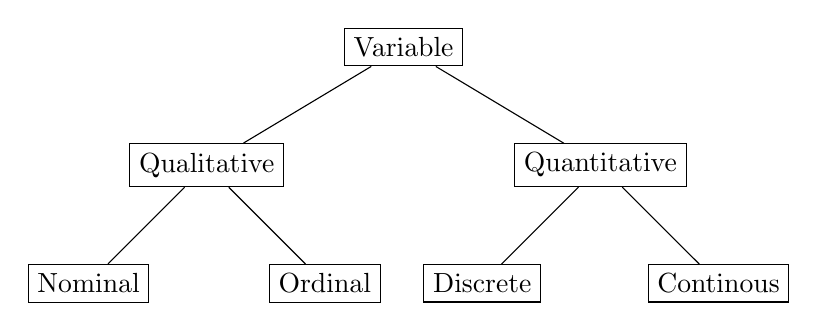
\begin{tikzpicture}
\tikzstyle{level 1}=[sibling distance=50mm]
  \tikzstyle{level 2}=[sibling distance=30mm]
  \tikzstyle{level 3}=[sibling distance=10mm]
	
  \node[rectangle,draw] {Variable}
    child {node[rectangle,draw] {Qualitative}
			child {node[rectangle,draw] {Nominal}}
			child {node[rectangle,draw] {Ordinal}}}
    child {node[rectangle,draw] {Quantitative}
      child {node[rectangle,draw] {Discrete}}
      child {node[rectangle,draw] {Continous}}};
\end{tikzpicture}

%\end{document}